\section{Reduce to 1D problem}

  The system (\ref{equ:model_system} - \ref{equ:model_functions}) can be reduced to a $1D$ problem. 
  
  %!% ADD HERE THE BASICS FOR THE TRAVELLING WAVE SCENARIO (HOMOGENOUS IC ON REGION BOUNDARY)
  
  Since the initial conditions are homogenous with respect to x, the x axis can be ignored and only the y-z axis is needed for visualization. Looking at Figure \ref{fig:visual}, the homoginity is clear.
   
  \begin{figure}[h!bt]
    \begin{center}
      \begin{tabular}{c c}
        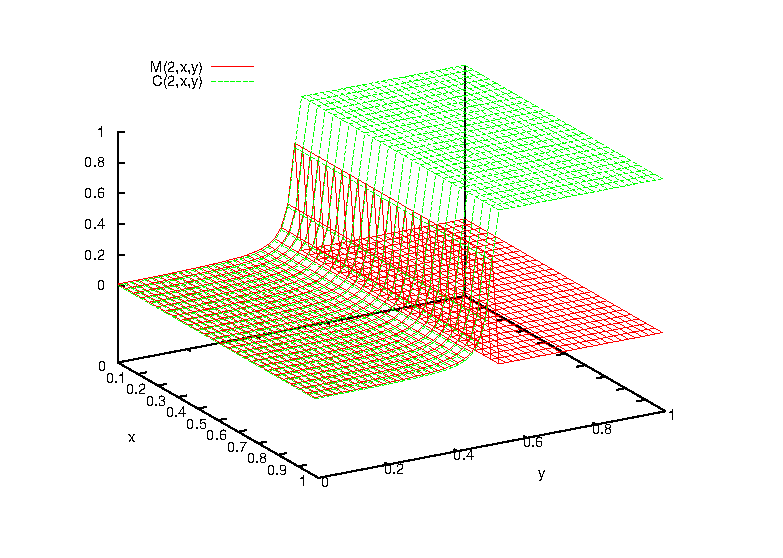
\includegraphics[scale=0.5]{view_3D.eps} &
        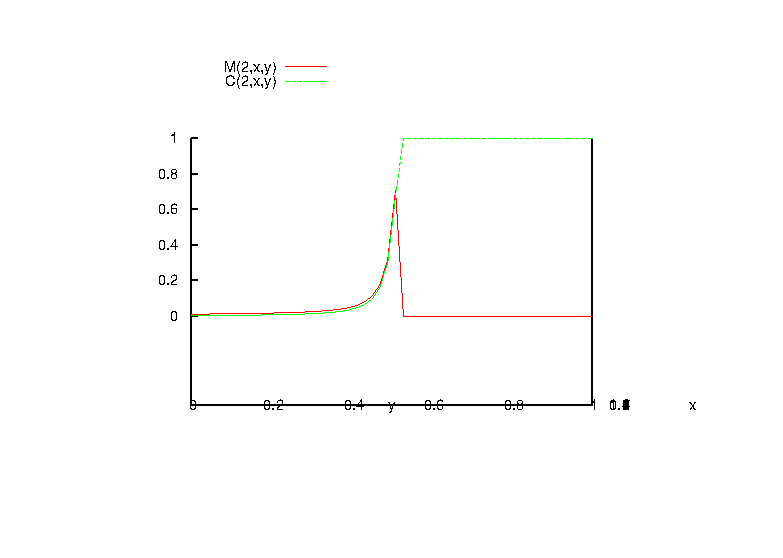
\includegraphics[scale=0.5]{view_psuedo2D.eps} \\
        (a) & (b) \\
      \end{tabular}
      \caption{Graph of (a) 3D view of $M(t,x,y)$ and $C(t,x,y)$, (b) Side profile view of $M(t,x,y)$ and $C(t,x,y)$ at $t=2$.} 
      \label{fig:visual}
    \end{center}
  \end{figure}
   
    This can be shown quantitatily by comparing the maximum and minimum values of M and C with respect to the x-axis (Figure \ref{fig:maxMin}). 
  \begin{figure}[h!bt]
    \begin{center}
        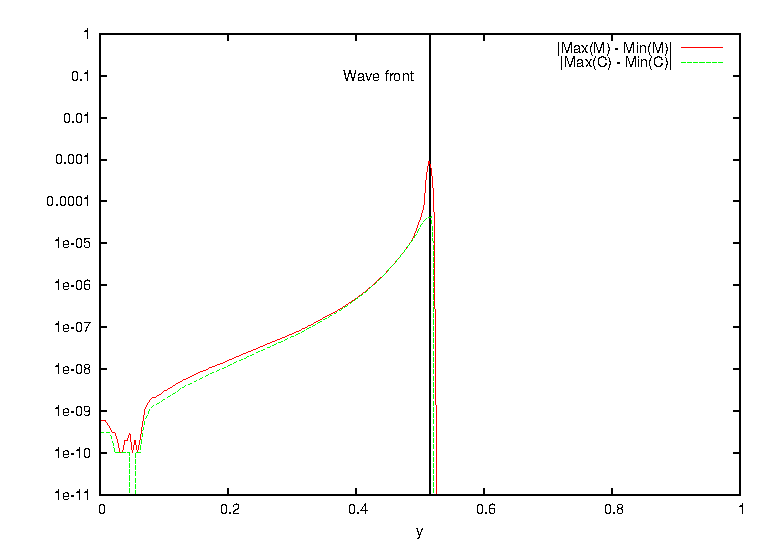
\includegraphics[scale=0.8]{maxMin_MC.eps}
      \caption{Graph of difference between max and min of M and difference between max and min of C.}
      \label{fig:maxMin}
    \end{center}
  \end{figure}

  The difference between the max and min remains constant with respect to time (Table \ref{tab:overTime}), this was calculated by,
  \begin{equation}
    \begin{aligned}
      \delta_M(t) &= \frac{1}{256}\sum_{i = 1}^n \left( \sup_{j \in (1,m)} M(x_i,y_j) - \inf_{k \in (1,m)} M(x_i,y_k) \right) \\
      \delta_C(t) &= \frac{1}{256}\sum_{i = 1}^n \left( \sup_{j \in (1,m)} C(x_i,y_j) - \inf_{k \in (1,m)} C(x_i,y_k) \right)   
    \end{aligned}
  \end{equation}
  
   \begin{table}
    \begin{center}
      \begin{tabular}{| c | c | c |} 
        \hline
        t & $\delta_M$ & $\delta_C$ \\
        \hline
        0.0 & 0.0 & 0.0037109375 \\
        0.5 &1.71577851563e-06 & 0.00371116503633\\
        1.0 &7.62408671875e-06 & 0.00371156747773\\
        1.5 &9.04633828125e-06 & 0.00371216829336\\
        2.0 &7.648728125e-06 & 0.00371311224609\\
        2.5 &2.58707890625e-06 & 0.00371457725742\\
        3.0 &0.00162623974609 & 0.00240237613672\\
        3.5 &5.35270417969e-05 & 7.24265101562e-05\\
        4.5 &1.07250539062e-05 & 2.12679726563e-05 \\
        5.0 &1.09254414063e-06 & 9.720734375e-06\\
        \hline
      \end{tabular}
      \caption{A table of values for $\delta_M(t)$ and $\delta_C(t)$}
      \label{tab:overTime}
    \end{center}
  \end{table}
   
   So by taking the average of the points along the $x$-axis we can get a 2D plot as seen in Figure \ref{fig:true2D}. 
   
 
   
 
    
  \begin{figure}[h!bt]
    \begin{center}
        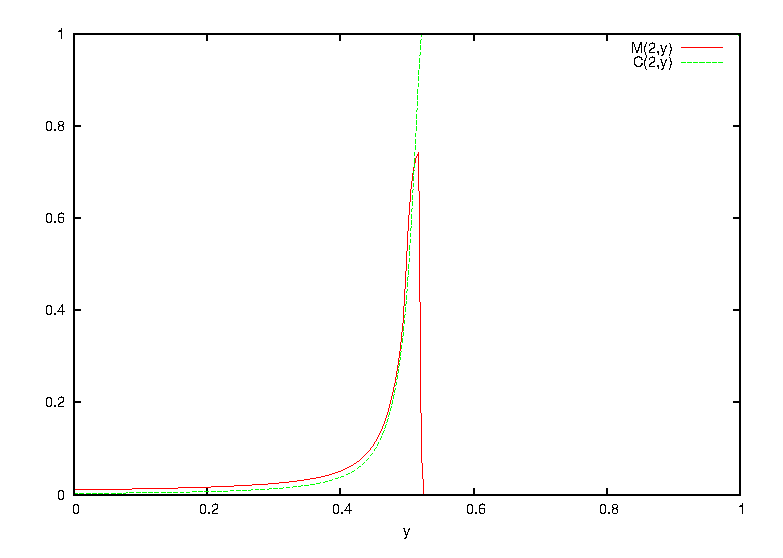
\includegraphics[scale=0.8]{view_2D.eps}
      \caption{Graph of M(2,y) and C(2,y), now reduced to a 2D plot.}
      \label{fig:true2D}
    \end{center}
  \end{figure}






